\part{Planejamento}

\chapter[Planejamento]{Planejamento}

\section{Descri\c{c}\~ao do problema}

\begin{figure}[H]
	\centering
	\label{FISHBONE}
		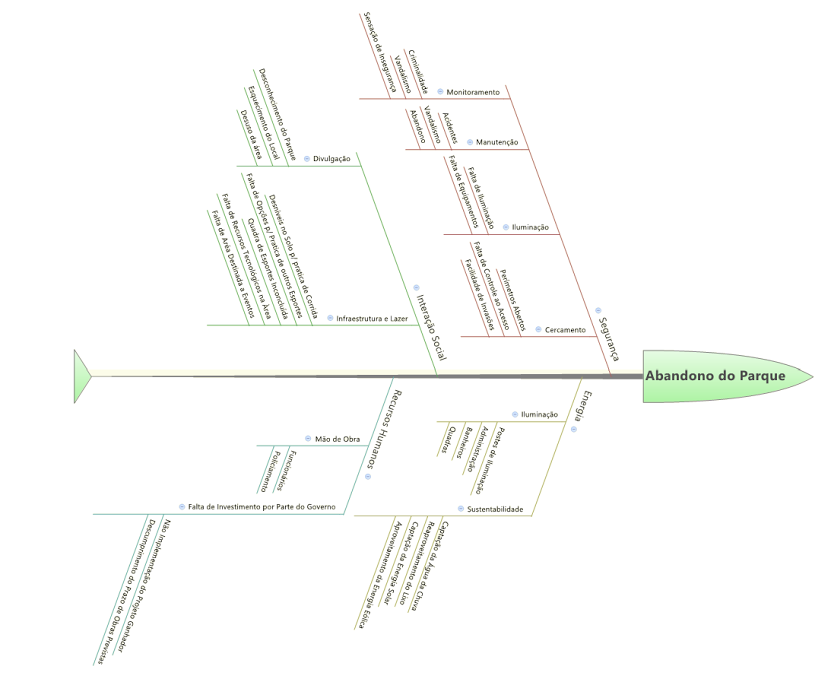
\includegraphics[keepaspectratio=true,scale=0.6]{planejamento/FISHBONE_complete.png}
	\caption{Fishbone do projeto.}
\end{figure}

Os problemas apresentados s\~ao descridos a seguir:

\subsection{Problemas encontrados}

\begin{itemize}
	\item Ilumina\c{c}\~ao: a ilumina\c{c}\~ao \'e um dos grandes problemas do parque. Sem uma ilumina\c{c}\~ao adequada a sensa\c{c}\~ao de seguran\c{c}a \'e m\'inima, dando condi\c{c}\~oes propicias ao crime e consequentemente diminuindo o n\'umero de frequentadores do parque.
	\item Falta de Monitoramento do Parque: o monitoramento do parque \'e quase nulo, muitos lugares estão sendo usados para pr\'aticas de crimes, passando a sensa\c{c}\~ao de abandono do parque com consequ\^encias similares a da falta de ilumina\c{c}\~ao, um bom monitoramento resolveria os problemas do parque, como tamb\'em o da popula\c{c}\~ao das imedia\c{c}\~oes da \'area patrulhada.
	\item Danos na cerca do parque: o cercamento do parque est\'a em condi\c{c}\~oes medianas de conserva\c{c}\~ao, mas possui buracos e em algumas \'areas ele \'e ausente propiciando invas\~oes do terreno, crimes, esconderijos para criminosos e degrada\c{c}\~ao ambiental.
	\item Falta de manuten\c{c}\~ao da infraestrutura: a manuten\c{c}\~ao do parque \'e prec\'aria, com brinquedos quebrados, cal\c{c}adas rachadas al\'em de problemas com a ilumina\c{c}\~ao, isso causa acidentes, evita a pr\'atica de esportes e prejudica o lazer. Solucionando este problema o parque ficaria em boas condi\c{c}\~oes para e uso, evitando reformula\c{c}\~oes do projeto, conservando assim o dinheiro e protegendo a fauna e flora local.
	\item Fonte n\~ao sustent\'avel de energia: n\~ao existe uma fonte sustent\'avel de fornecimento de energia para o parque.
	\item Lixo produzido nos banheiros por usu\'arios e pela administra\c{c}\~ao: o lixo produzido deve ter uma devida destina\c{c}\~ao para n\~ao danificar o local. Este fator \'e extremamente importante, uma vez que o parque \'e considerado reserva ambiental.
	\item A falta de atratividade do parque: a falta de atratividade do parque devido \`a falta de op\c{c}\~ao de recrea\c{c}\~ao, falta de intera\c{c}\~ao entre as pessoas, al\'em de todos os problemas estruturais b\'asicos.
\end{itemize}

\subsection{Quem s\~ao os afetados pelos problemas encontrados}
	
	Os problemas listados podem afetar diretamente ou indiretamente v\'arios p\'ublicos, dentre eles est\~ao a comunidade vizinha ao parque, as crian\c{c}as e jovens que estudam em escolas pr\'oximas. Pessoas que procuram um local para praticar esportes ao ar livre e ter op\c{c}\~oes de lazer e intera\c{c}\~ao social.
	Outro grupo que possivelmente frequenta o parque s\~ao os moradores de rua e habitantes de moradias n\~ao regulamentadas. Sendo assim, policiais, ONG's e agentes governamentais necessitar\~ao estarem presentes.
	Al\'em de toda a comunidade ao redor do parque, que n\~ao necessariamente seja composta apenas por moradores. Incluindo comerciantes, universit\'arios, funcion\'arios do setor p\'ublico em geral que busquem um local de lazer para a os intervalos de trabalho e o fim do expediente.
	Contudo, o local tamb\'em \'e apropriado para receber eventos a n\'ivel distrital devido a sua representatividade e ao espa\c{c}o dispon\'ivel. Afirmando sua caracter\'istica sustent\'avel e ecol\'ogica, o parque buscar\'a repercutir e atrair cada vez mais pessoas.
	
\subsection{Impactos}

Todo problema gera impactos e \'e necess\'ario identificar cada um deles para poder priorizar solu\c{c}\~oes para as causas mais graves. Em seguida s\~ao apresentados impactos observados com o abandono do Parque Urbano do Gama e seus problemas decorrentes:

\begin{itemize}
	\item N\~ao aproveitamento do potencial de atividades que o parque pode oferecer;
	\item A popula\c{c}\~ao n\~ao possui responsabilidade em cuidar, cobrar as autoridades locais;
	\item Ambiental: na forma de polui\c{c}\~ao visual, degrada\c{c}\~ao ambiental, solo, len\c{c}ol fre\'atico;
	\item Presen\c{c}a de usu\'arios de entorpecentes;
	\item Inseguran\c{c}a;
	\item Crimes nas redondezas;
	\item Degrada\c{c}\~ao do patrim\^onio p\'ublico;
	\item Degrada\c{c}\~ao ambiental;
	\item Acidentes;
\end{itemize}

\subsection{5W2H}

A primeira atividade realizada pelo grupo foi responder o 5W2H para ter no\c{c}\~oes iniciais das motiva\c{c}\~oes, causas entre outras informa\c{c}\~oes relacionadas ao projeto. A seguir est\~ao as respostas estabelecidas pelo grupo.

\begin{itemize}
	\item What? (O que ser\'a entregue?): ser\'a entregue um projeto de revitaliza\c{c}\~ao de um parque urbano, em que ser\'a utilizada a tecnologia como principal ferramenta.
	\item Why? (Por qu\^e est\'a sendo feito?): Est\'a sendo realizado devido a atual inutiliza\c{c}\~ao de um espa\c{c}o p\'ublico que possui grande potencial de servir a comunidade vizinha, com o prop\'osito de uma maior comodidade e incentivo ao acesso a partir das aplica\c{c}\~oes tecnol\'ogicas, o que seria um diferencial em vista de outros parques.
	\item Where? (Onde ser\'a feito/ entregue/ utilizado?): Ser\'a feito no parque vivencial urbano localizado na cidade do Gama do Distrito Federal. Uma regi\~ao de cerrado, n\~ao preservado, em que h\'a invas\~oes ilegais, pista de aeromodelismo, problemas de seguran\c{c}a e limpeza.
	\item When? (Quando ser\'a feito/ entregue?): O projeto tem dura\c{c}\~ao de tr\^es meses, tendo como data final de entrega dia 22 de junho de 2015.
	\item Who? (Quem o far\'a?): A realiza\c{c}\~ao deste projeto ser\'a pelos alunos de gradua\c{c}\~ao dos cursos de Engenharia conciliada com empresas interessadas, o Governo do Distrito Federal, \textit{stakeholders} em geral, como a popula\c{c}\~ao interessada.
	\item How? (Como ser\'a realizado?): Ser\'a realizado a partir de pesquisas acerca do tema, reuni\~oes, debates de ideias e utiliza\c{c}\~ao de metodologias de gerenciamento de projetos, como o \textit{SCRUM} e ferramentas de comunica\c{c}\~ao, como o \textit{Trello}.
	\item How much? (Quanto custar\'a?): Analisando, primeiramente a hora-homens trabalhadas, pode-se estimular um valor.

Determinando: 
\begin{itemize}
        \item 9 pessoas ganhando 6 mil
	\item 8 pessoas ganhando 9 mil
	\item 8 pessoas ganhando 4 mil
\end{itemize}

semanalmente 8 horas trabalhadas --- um m\^es 32 horas
acrescentando 25\% de risco

Tem-se : R\$ 197500,00 o que corresponde em hora/m\^es a R\$ 246,32.
\end{itemize}

\section{Justificativa}

A principal motiva\c{c}\~ao do projeto consiste no abandono do parque pela popula\c{c}\~ao e pelo governo, resultando na falta de aproveitamento do parque, em seu potencial social, ecológico e turístico. Com a devida revitaliza\c{c}\~ao, o parque poderia acrescentar op\c{c}\~oes de intera\c{c}\~ao social para o Gama, favorecendo os moradores da cidade e a todos que possam frequent\'a-la.
Devido a essa motiva\c{c}\~ao o que se encontra na realidade do parque s\~ao problemas de seguran\c{c}a, limpeza, o que acarreta baixa especula\c{c}\~ao imobili\'aria em torno e invas\~oes. 

\section{Definição de Escopo do Projeto}

	O projeto consiste em desenvolver soluções tecnológicas para o parque do Urbano e Vivencial do Gama. Foi observado que o parque apresenta uma grande extensão, de aproximadamente 52 mil metros quadrados. No entanto, não se mostrou viável criar soluções que estejam presentes por toda a extensão do parque. A primeira restrição que foi adotada foi com relação ao processo que está em andamento por parte da Administração Regional. Através de visitas ao local foi possível obter a planta entre outras informações sobre o projeto implementado. Dessa forma, caso o projeto desenvolvido na disciplina de Projeto Integrador 1 se torne viável, seria interessante apresentá-lo para possíveis steakholders. 

	Dentro das delimitações do projeto estipulou-se um número de visitantes em dias de alta movimentação, como os fins de semana, em torno de 1300 pessoas. Este número foi embasado em uma comparação com o Parque de Águas Claras e uma combinação desse valor com o número de visitantes esperados devido ao espaço Lazer- Multimídia. 
Dentro dos subsistemas também foram estipuladas delimitações para o projeto. 
	
	O espaço de interação social está sendo projetado para suportar um número de até 1000 pessoas. Dentro deste espaço terão 30 bicicletas ergométricas. A energia gerada pelas mesmas será consumida simultaneamente, sem o armazenamento de energia. 
	
	A energia gerada pelos painéis fotovoltáicos será armazenada para alimentar os mesmos durante o período que a luz ambiente for menor, no geral no período noturno. Os outros equipamentos do parque, que não incluam a iluminação geral e nem o espaço interativo serão alimentados pela energia elétrica da rede, um consumo estimado em torno de  2054,57 kWh. A Segurança projetada para o parque tem foco na segurança das pessoas e patrimônio físico, não abrangendo a segurança ambiental. Consequentemente uma das soluções abordadas é o cercamento do parque. O perímetro estipulado para tal é de 3342,29 metros. 

\section{Objetivos}

Nesta se\c{c}\~ao est\~ao descritos os objetivos que devem ser atingidos ao final deste projeto.

\subsection{Objetivo Geral}

Buscar solu\c{c}\~oes tecnol\'ogicas para aumentar a atratividade do parque urbano e vivencial do Gama - DF, aumentando a intera\c{c}\~ao social por parte da popula\c{c}\~ao, fornecendo lazer, sustentabilidade, seguran\c{c}a e preservando a natureza do local. 

\subsection{Objetivos Espec\'{\i}ficos}

Integrar os cursos de engenharia: automotiva; aeroespacial; energia; eletr\^onica e software em que situam os alunos a projetar, colocar em pr\'atica conceitos estudados. 
Apresentar um planejamento de como executar a revitaliza\c{c}\~ao tecnol\'ogica. Relacionar os aspectos f\'isicos e burocr\'aticos que se encontram na regi\~ao atualmente, e as obras j\'a iniciadas pela Administra\c{c}\~ao Regional do Gama; com as legisla\c{c}\~oes distritais que limitam no tocante ao meio ambiente, a popula\c{c}\~ao vizinha e os impactos urbanos. 

\section{Metodologia}

\subsection{Estrutura Organizacional}

O grupo foi subdividido em grupos menores visando resolver os principais problemas encontrados no parque.

\begin{figure}[H]
	\centering
	\label{Estrutura Organizacional}
		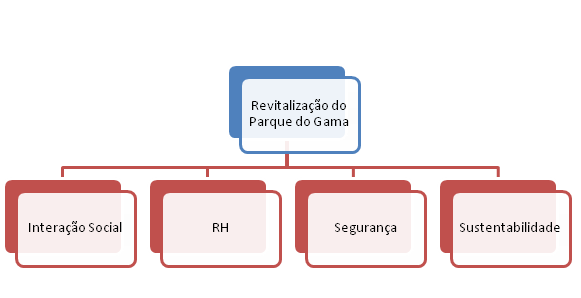
\includegraphics[keepaspectratio=true,scale=1.0]{planejamento/EstruturaOrganizacional.png}
	\caption{Esquem\'atico da divis\~ao dos grupos do projeto.}
\end{figure}

\begin{itemize}
    \item Sustentabilidade: Esse grupo visa a sustentabilidade do parque, preocupando-se com as quest\~oes ambientais.
	\item Seguran\c{c}a: Esse grupo visa tornar o ambiente seguro para visita\c{c}\~ao.
	\item Recursos Humanos - Controle: Esse grupo visa administrar os entreg\'aveis, organiza a documenta\c{c}\~ao, controla a integra\c{c}\~ao de todo o grupo.
	\item Interação social: Esse grupo visa tornar o parque mais atrativo de forma que possa interrelacionar a população do Gama e região.
\end{itemize}

\subsection{Gerenciamento dos Recursos Humanos}

Esta se\c{c}\~ao mostra como os integrantes do projeto foram alocados e quais as suas respectivas fun\c{c}\~oes.

\subsubsection{Pap\'eis e Responsabilidades}
Esta subse\c{c}\~ao mostra os pap\'eis dos integrantes do projeto e quais as suas respectivas responsabilidades.

\begin{table}[H]
\caption{Descri\c{c}\~ao das atividades de cada um dos membros.} 
\begin{center}
\begin{tabular}{|p{3cm}|p{4cm}|p{8cm}|} \hline

Cargo &Nome &Fun\c{c}\~ao\\ \hline 

Gerente Geral &Let\'icia Barros &Planejar atividades coletivas, bem como estabelecer t\'opicos de discuss\~ao para as reuni\~oes presenciais. Al\'em disso, deve acompanhar o desenvolvimento dos subgrupos e buscar a integra\c{c}\~ao entre eles para que todos possam seguir processos espec\'ificos que devem se interrelacionar ao longo do projeto buscando um melhor desempenho geral \\ \hline

Subgerentes &Let\'icia Munhoz (Intera\c{c}\~ao Social)  Helton (Seguran\c{c}a)  Renner (Sustentabilidade)  Ebenezer (RH) &Planejar reuni\~oes menores para cada um dos seus grupos, designar tarefas para cada um dos seus membros e averiguar a qualidade dos artefatos, no tempo esperado e repassar essas informa\c{c}\~oes para que a gerente geral e os demais alunos possam acompanhar o que est\'a sendo feito \\ \hline

Pesquisadores de sustentabilidade &Lucas Rossi, Henrique, Daniel, Matheus Coelho, Bernardo &Trabalhar de forma a encontrar as solu\c{c}\~oes mais vi\'aveis para gerar energia para as atividades do parque sem desrespeitar a legisla\c{c}\~ao vigente \\ \hline
Pesquisadores de Intera\c{c}\~ao Social &Eduardo, Fernanda, Diogo, Ruan e Rodrigo &Realizar o acompanhamento da popula\c{c}\~ao do Gama e poss\'iveis interessados na reforma do parque para buscar formas de aumentar a atratividade do local \\ \hline 

Pesquisadores de seguran\c{c}a &Divino, Matheus Alves, David, Higor, Victor Hugo, Victor Henrique &Projetar mecanismos para controlar a seguran\c{c}a do parque de forma a oferecer um ambiente seguro para visita\c{c}\~ao \\ \hline

Pesquisadores de controle &Luciana, Lu\'is e Marcos Gois. &Esse grupo visa administrar os entreg\'aveis, organiza a documenta\c{c}\~ao, controla a integra\c{c}\~ao de todo o grupo. \\ \hline

 \end{tabular}
\end{center}
\end{table}

\subsection{Plano de Comunica\c{c}\~ao}

Para a comunica\c{c}\~ao foram utilizadas v\'arias plataformas, como descrito a seguir:

 \textit {Facebook}: foi a primeira ferramenta utilizada e o grupo foi criado na primeira reuni\~ao do projeto. Inicialmente documentos eram compartilhados utilizando essa ferramenta, o que n\~ao se mostrou muito eficaz pela falta de recursos para organizar os arquivos e pelo site ser bloqueado na Universidade. No entanto, a ferramenta ainda \'e utilizada para avisos r\'apidos sobre atividades. 

\textit{Whatsapp}: esta ferramenta foi utilizada para aumentar o n\'ivel de intera\c{c}\~ao dos membros e tamb\'em serve para avisos gerais, como comunicar que alguma documenta\c{c}\~ao deve ser atualizada.

 \textit{Google Drive}: ferramenta mais utilizada pelo grupo. Ela serve como banco de dados. Todas as refer\^encias e resultados de pesquisas tem sua documenta\c{c}\~ao organizada nessa plataforma. Ela se mostrou atrativa por poder ser melhor organizada, oferecer um grande espa\c{c}o de mem\'oria e possibilidade de edi\c{c}\~ao de documentos em grupo.

 \textit{Trello}: esta ferramenta foi utilizada com o \'unico intuito de ser um local de acesso r\'apido para a averigua\c{c}\~ao do andamento das atividades propostas.

\begin{figure}[H]
	\centering
	\label{comunicacao}
		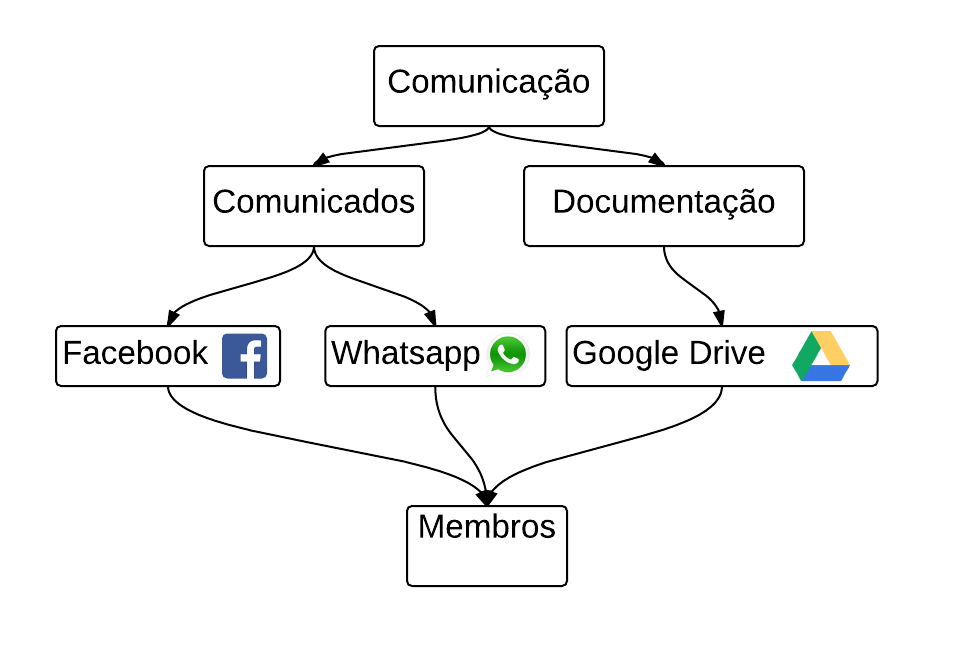
\includegraphics[keepaspectratio=true,scale=0.7]{planejamento/comunicacao.png}
	\caption{Esquem\'atico de comunica\c{c}\~ao}
\end{figure}

\subsection{Gerenciamento do Tempo}

A gest\~ao do tempo partiu das datas dos Pontos de Controle (PC1, PC2 e PC3), Atrav\'es dessas datas foram estipulados os pontos cr\'iticos de entregas do projeto. Para relacionar as atividades fundamentais a serem realizadas pela equipe foi feita uma rela\c{c}\~ao entre as atividades da metodologia, que \'e descrita na pr\'oxima se\c{c}\~ao e os entreg\'aveis da EAP (Estrutura Anal\'itica de Projeto).
Os prazos para realiza\c{c}\~ao das atividades iniciais foram realizados de acordo com as necessidades do projeto, como constru\c{c}\~ao de artefatos e realiza\c{c}\~ao de tarefas. 
A partir da sprint 0 foi abordado o prazo para realiza\c{c}\~ao da sprint entre os subgerentes e a gerente de projeto que foi definido de uma semana. Essa sprint ser\'a a sprint modelo para que se possa tomar conhecimento da real necessidade de tempo que a equipe levar\'a para realizar as atividades demandadas. Com base nessas informa\c{c}\~oes foi constru\'ido no final da macro atividade - Manter Planejamento - a primeira vers\~ao do cronograma. A primeira vers\~ao do documento segue em anexo no final do relat\'orio .

\subsection{Desenvolvimento de Projeto/ Metodologia}

Para selecionar uma metodologia para apoiar o desenvolvimento foi analisado o ambiente do projeto, rela\c{c}\~ao entre a parte interna da equipe, rela\c{c}\~ao entre equipe e cliente e o impacto sobre os \textit{stakeholders}. 
	O projeto apresenta requisitos inst\'aveis, tamb\'em como o surgimento de novos requisitos durante a execu\c{c}\~ao do projeto, essas caracter\'isticas s\~ao uma das que mais impactaram a sele\c{c}\~ao da metodologia \textit{Scrum}. Tamb\'em o contato com o cliente ocorre de forma simples e pode ser estabelecida semanalmente. O cliente identificado na identifica\c{c}\~ao dos \textit{stakeholders} \'e a Administra\c{c}\~ao do Gama-DF e devido a proximidade geogr\'afica de alguns integrantes da equipe de desenvolvimento com a Administra\c{c}\~ao do Gama acabou influenciando a sele\c{c}\~ao da metodologia. 
Para adapta\c{c}\~ao da metodologia de acordo com as reais necessidades do projeto, primeiramente foi utilizado o SAFe (\textit{Scaled Agile Framework}) que fornece uma estrutura para aplica\c{c}\~ao de metodos \'ageis para desenvolvimento de projetos. A partir deste \textit{framework} foi constru\'ido um processo de desenvolvimento que ser\'a aplicado no projeto de acordo com as necessidades da equipe. O processo foi modelado utilizando o Bizagi Modeler, abaixo segue a descrição do processo modelado

\begin{landscape}
\subsubsection{Visão Completa do Processo}

\begin{figure}[H]
	\centering
	\label{Visão geral do processo modelado}
		\includegraphics[keepaspectratio=true,scale=0.9,angle=360]{processo/ProcessoCompleto.png}
	\caption{Visão geral do processo modelado.}
\end{figure}
\end{landscape}
\subsubsection{Iniciar Projeto}

\begin{figure}[H]
	\centering
	\label{Visão do processo Iniciar Projeto}
		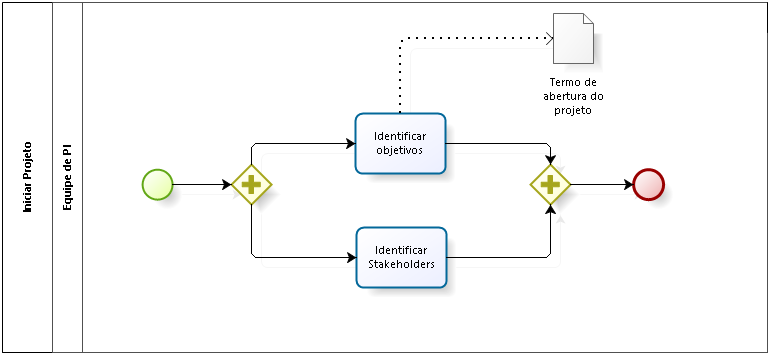
\includegraphics[keepaspectratio=true,scale=0.7,angle=360]{processo/IniciarProjeto.png}
	\caption{Visão do processo Iniciar Projeto.}
\end{figure}

No processo iniciar projeto é onde ocorre o levantamento das informações fundamentais para iniciação do projeto. 

\begin{enumerate}
	\item \textbf{Identificar objetivos:} 
		Identificar todos os objetivos necessários para realização do termo de abertura do projeto, é nessa atividade que esse artefato é construído.
	\item \textbf{Identificar stakeholders:}
		Identificar todas as pessoas e organizações que estão interessadas ou serão impactadas com o desenvolvimento do projeto. 
\end{enumerate}

\begin{itemize}
	\item \textbf{Artefatos:}
		\begin{itemize}
		\item Termo de abertura do projeto: Documento com as definições fundamentais para definição/estruturação do trabalho. 
		\end{itemize}
\end{itemize}

\subsubsection{Manter Planejamento}

No processo Manter Planejamento é onde ocorre as atividades de identificação/conhecimento do problema ao qual o projeto será realizado, também ocorre a identificação dos requisitos necessários para o projeto e o planejamento iterativo do projeto. 

\begin{landscape}
\begin{figure}[H]
	\centering
	\label{Visão do processo Manter Planejamento}
		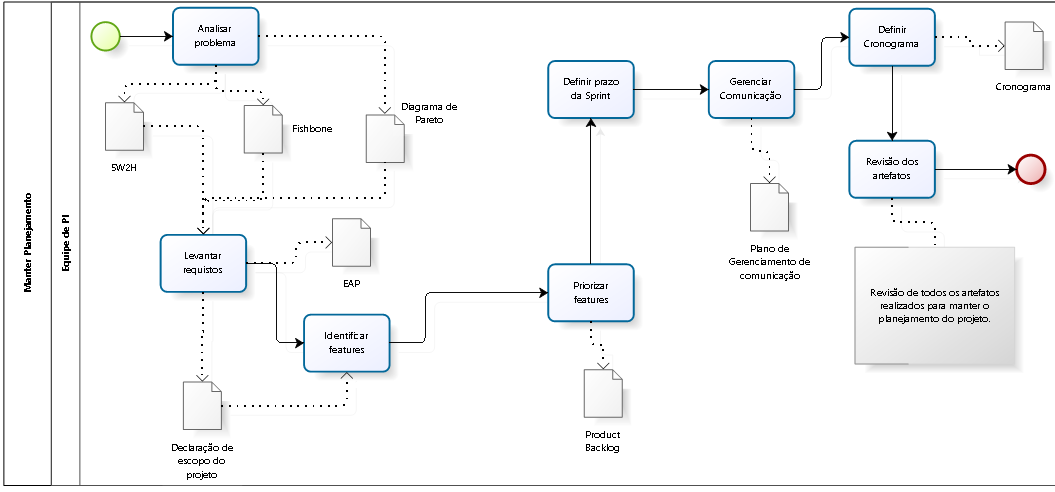
\includegraphics[keepaspectratio=true,scale=0.9,angle=360]{processo/manterPlanejamento.png}
	\caption{Visão do processo Manter Planejamento.}
\end{figure}
\end{landscape}

\begin{enumerate}
	\item \textbf{Analisar problema:}  
	Aplicação de técnicas de análise do problema com o intuito de tomar conhecimento das reais necessidades dos stakeholders, nesta atividade é aplicada a técnica do fishbone, diagrama de pareto e o 5W2H.
	\item \textbf{Levantar requisitos:} 
	Atividade ao qual é levantado os requisitos necessários de todo o projeto, sobre o olhar das principais necessidades do cliente. Requisitos não funcionais do projeto são levatados, mas o foco da atividade é levantar as principais características tecnológicas que podem ser aplicadas ao projeto.
	\item \textbf{Identificar features:} 
	Identificação das principais características que o parque necessita para prover de uma maior interação com a sociedade. 
	\item \textbf{Priorizar features:} 
	Definir quais são as características mais importantes de serem implementadas no parque.
	\item \textbf{Definir prazo da sprint:} 
	Reunião com todos os membros do projeto com o intuito de determinar o intervalo em dias/semanas das sprints do projeto. 
	\item \textbf{Gerenciar comunicação:} 
	Reunião para definir quais são as ferramentas de comunicação que podem ser implemnetadas no projeto e desenvolver um planejamento de comunicação.
	\item \textbf{Definir cronograma:} 
	Construir cronograma de acordo com os marcos do projeto e os artefatos entregáveis. 
	\item \textbf{Revisão dos artefatos:} 
	Realizar revisão de todos os artefatos gerados no fluxo de manter planejamento. 
\end{enumerate}

\begin{itemize}
	\item Artefatos
	\begin{itemize}
		\item 5W2H
		\item Fishbone
		\item Diagrama de pareto
		\item EAP
		\item Declaração de escopo do projeto
		\item Product Backlog 
		\item Plano de gerenciamento de comunicação
		\item Cronograma do projeto
	\end{itemize}
\end{itemize}

\subsubsection{Planejar Sprint}

É uma reunião que seu objetivo é fazer o planejamento da Sprint. Na primeira parte a equipe do projeto faz outra atividade que visa tornar mais claro o que ainda deve ser feito esses requisitos devem ser prioritariamente levantados a partir das features priorizadas na atividade anterior.

\begin{figure}[H]
	\centering
	\label{Visão do processo Planejar Sprint}
		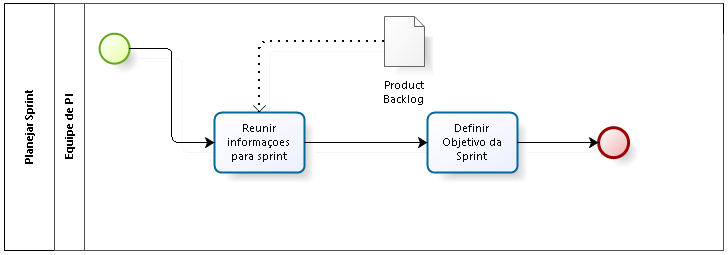
\includegraphics[keepaspectratio=true,scale=0.9,angle=360]{processo/planejarSprint.png}
	\caption{Visão do processo Planejar Sprint.}
\end{figure}

\begin{enumerate}
	\item \textbf{Reunir informações para sprint:} 
	Analisar o product backlog e identificar quais características do projeto tem maior relevânica de ser projetada sobre o olhar das necessidades do usuário do parque do Gama-DF, através destas informações é definido o que será projetado na sprint. 
	\item \textbf{Definir objetivo da sprint:} 
	Reunião para identificar onde a equipe do projeto deseja chegar ao final da sprint, quais são as metas desejadas. 
\end{enumerate}

\begin{itemize}
	\item Artefato
	\begin{itemize}
		\item Backlog da sprint
		O backlog da sprint possui as características do projeto que serão pesquisadas/projetadas durante a execução da sprint. 
	\end{itemize}
\end{itemize}


\subsubsection{Controlar Sprint}

Essa atividade tem como objetivo acompanhar o andamento da Sprint, o subgerente de Recursos Humanos e Controle é responsável por avaliar a produção do time.

\begin{figure}[H]
	\centering
	\label{Visão do processo Controlar Sprint}
		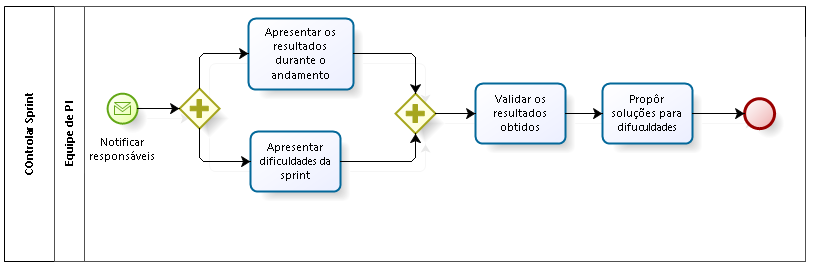
\includegraphics[keepaspectratio=true,scale=0.7,angle=360]{processo/controlarSprint.png}
	\caption{Visão do processo Controlar Sprint.}
\end{figure}

\begin{enumerate}
	\item \textbf{Apresentar resultados durante o andamento:}
	Essa atividade tem como objetivo mostrar os resultados obtidos pelo time durante a execução da sprint ao subgerente de Recursos Humanos e Controle.
	\item \textbf{Apresentar dificuldades da sprint:}
	Apresentar dificuldades durante a execução da Sprint ao subgerente de Recursos Humanos e Controle.
	\item \textbf{Validar os resultados obitidos:}
	O subgerente de Recursos Humanos e Controle valida se o que o time está executando na Sprint e de forma correta.
	\item \textbf{Propôr soluções para as dificuldades:}
	O subgerente de Recursos Humanos e Controle propõe soluções para o time de acordo com as informações apresentadas.
\end{enumerate}

\subsubsection{Executar Sprint}

Para a atividade de executar a Sprint temos que consultar o product backlog e é selecionado as características mais relevantes do projeto para serem pesquisadas/projetadas. Essa é a atividade onde são levantadas as soluções para o problema do parque urbano do Gama-DF

\begin{figure}[H]
	\centering
	\label{Visão do processo Executar Sprint}
		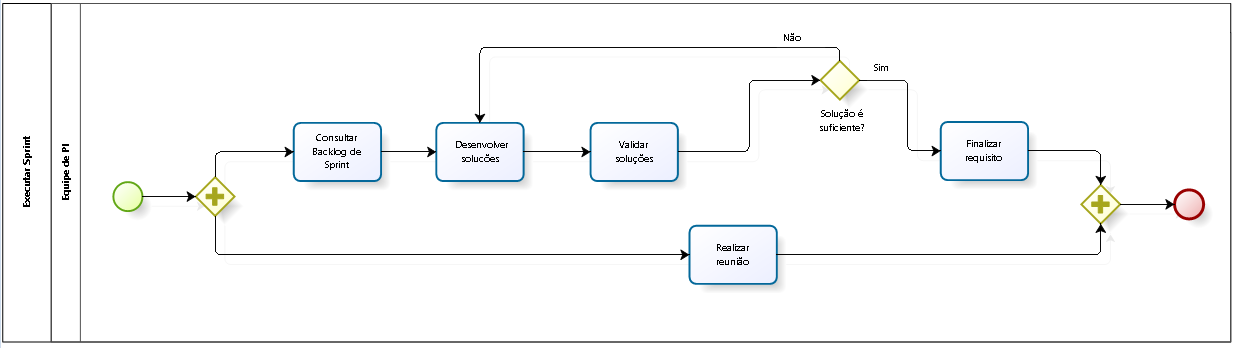
\includegraphics[keepaspectratio=true,scale=0.5,angle=360]{processo/executarSprint.png}
	\caption{Visão do processo Executar Sprint.}
\end{figure}

\begin{enumerate}
	\item \textbf{Consultar sprint backlog:}
	Nessa atividade o time deve consultar as caraterísticas do projeto definidas para a Sprint.
	\item \textbf{Desenvolver solução:}
	Aplicar medidas técnicas de desenvolvimento para prover solução.
	\item \textbf{Validar soluções:}
	O subgerente e o gerente verifica se a solução implementada atende sua necessidade real do parque urbano do Gama-DF. 
	\item \textbf{Finalizar requisito:}
	Finalizar requisito do projeto ao executado na sprint, nesta atividade é realizada a validação da solução com todos os integrantes do projeto. 
	\item \textbf{Realizar reunião}
	Reunião realizada durante os encontros para desenvolvimento do projeto, com intuito de prover uma integração de todas as equipes do projeto. 
\end{enumerate}

\subsubsection{Revisar Sprint}

Está é uma reunião realizada no final da sprint. Tem como Objetivo apresentar o que  a equipe fez durante a sprint e apresentar o produto para os Subgerentes e o gerente. 

\subsubsection{Realizar Retrospectiva}
Tem como objetivo avaliar o que deu certo e errado durante a sprint, e fazer os ajustes possíveis  para a proxima Sprint.

\subsection{Atualizar backlog}
Depois de executada a Sprint é realizada a atualização do backlog de programa onde pode ser detectado novos requisitos que refletem mudanças no sistema, eles poderão ser propostos nesta atividade e analisados e validados na (primeira atividade do fluxo de planejar Sprint: "Reunir informações para sprint") para que a mudança seja consistente e não impacte de maneira negativa a solução do projeto. Isso garante que as mudanças sejam realizadas e implementadas com sucesso, sem que haja perda na qualidade da solução do projeto.

\section{Fundamenta\c{c}\~ao Te\'orica}

\subsection{Planejamento de ilumina\c{c}\~ao}

Usando estruturas e materiais que al\'em de terem um baixo consumo de energia e pouco impacto ambiental em sua instala\c{c}\~ao possuem efici\^encia suficiente para atender as demandas por seguran\c{c}a da regi\~ao e dos usu\'arios do parque. Esta se mostrou a melhor proposta para  inibir atividades criminosas no local no per\'iodo da noite. Pois, iluminando o local e consequentemente as localidades pr\'oximas \`a sensa\c{c}\~ao de seguran\c{c}a ser\'a maior para os usu\'arios do parque (principalmente os praticantes de esportes) al\'em de inibir pr\'aticas il\'icitas dentro e nas imedia\c{c}\~oes da \'area iluminada.

\subsection{Planejamento ou projeto de monitoramento}

Procurar parceria com a pol\'icia militar da cidade do Gama ou de algum \'org\~ao p\'ublico que est\'a respons\'avel pela manuten\c{c}\~ao da ordem p\'ublica, com possibilidade de contrata\c{c}\~ao de uma empresa privada, al\'em de claro uma nova log\'istica de monitoramento interno com utiliza\c{c}\~ao de estruturas est\'aticas e moveis respectivamente, com a intercomunica\c{c}\~ao entre cada vi\'es de monitoramento (interno e externo), determinar um hor\'ario de funcionamento do parque e fech\'a-lo ap\'os esse per\'iodo para evitar crimes (entre eles ambientais) dentro do terreno do parque, colaborando assim com um bom funcionamento do parque, aumentar a movimenta\c{c}\~ao al\'em de ajudar a diminuir a criminalidade nas imedia\c{c}\~oes da \'area, preservando a integridade do parque e da popula\c{c}\~ao pr\'oxima. Contratar uma empresa para que sejam feita a manuten\c{c}\~ao constante do cercamento. Para que se tenha uma manuten\c{c}\~ao constante do parque \'e necess\'ario integrar empresas p\'ublicas e privadas, dessa forma \'e poss\'ivel garantir que todos os setores do parque recebam a devida manuten\c{c}\~ao, seja em uma \'area mais comum como, por exemplo, encanamento e distribui\c{c}\~ao de \'agua que pode ser feito por uma empresa p\'ublica, ou numa \'area mais espec\'ifica como a eletr\^onica de monitoramento que pode ser realizado por uma empresa privada.
	
	Utilizar empresas p\'ublicas e privadas seria a melhor op\c{c}\~ao para manter a manuten\c{c}\~ao no parque, pois existem diversos setores que necessitam de aten\c{c}\~ao. Na parte estrutural t\^em-se a manuten\c{c}\~ao do cercamento, das cal\c{c}adas ao redor do parque e do circuito de \textit{cooper} como exemplos, na parte de monitoramento, a manuten\c{c}\~ao das c\^ameras e dos softwares que fazem esse trabalho. Ou seja, seria necess\'ario ter empresas que atuam em diversas \'areas de conhecimento, isso justifica o porqu\^e de se usar empresas p\'ublicas e privadas.

\subsection{Postes com placa solar para abastecimento pr\'oprio}

Utiliza\c{c}\~ao de postes de ilumina\c{c}\~ao que possuem em sua parte superior uma placa fotovoltaica que capta a radia\c{c}\~ao solar e transforma em energia, que \'e armazenada em baterias no poste. Cada poste \'e um sistema isolado, ou seja, n\~ao conectado com a rede, sendo assim, uma falha em um deles n\~ao afeta os outros.

\subsection{Turbinas de vento para gera\c{c}\~ao de energia el\'etrica.}

A energia e\'olica - produzida a partir da for\c{c}a dos ventos - \'e abundante, renov\'avel, limpa e dispon\'ivel em muitos lugares. Essa energia \'e gerada por meio de aerogeradores, nas quais a for\c{c}a do vento \'e captada por h\'elices ligadas a uma turbina que aciona um gerador el\'etrico. A quantidade de energia transferida \'e em fun\c{c}\~ao da densidade do ar, da \'area coberta pela rota\c{c}\~ao das p\'as (h\'elices) e da velocidade do vento. \\ 

A avalia\c{c}\~ao t\'ecnica do potencial e\'olico exige um conhecimento detalhado do comportamento dos ventos. Os dados relativos a esse comportamento - que auxiliam na determina\c{c}\~ao do potencial e\'olico de uma regi\~ao - s\~ao relativos \`a intensidade da velocidade e \`a dire\c{c}\~ao do vento. Para obter esses dados, \'e necess\'ario tamb\'em analisar os fatores que influenciam o regime dos ventos na localidade do empreendimento. Entre eles pode-se citar o relevo, a rugosidade do solo e outros obst\'aculos distribu\'idos ao longo da regi\~ao. \\ 

Para que a energia e\'olica seja considerada tecnicamente aproveit\'avel, \'e necess\'ario que sua densidade seja maior ou igual a 500 W/m$^{2}$, a uma altura de 50 metros, o que requer uma velocidade m\'inima do vento de 7 a 8 m/s \cite{johansson1993renewable} . Segundo a Organiza\c{c}\~ao Mundial de Meteorologia, o vento apresenta velocidade m\'edia igual ou superior a 7 m/s, a uma altura de 50 m, em apenas 13\% da superf\'icie terrestre. Essa propor\c{c}\~ao varia muito entre regi\~oes e continentes. \\

Quanto \`a aplica\c{c}\~ao desse tipo de energia no Brasil, pode-se dizer que as grandes centrais e\'olicas podem ser conectadas \`a rede el\'etrica uma vez que possuem um grande potencial para atender o Sistema Interligado Nacional (SIN). As pequenas centrais, por sua vez, s\~ao destinadas ao suprimento de eletricidade a comunidades ou sistemas isolados, contribuindo para o processo de universaliza\c{c}\~ao do atendimento de energia. Em rela\c{c}\~ao ao local, a instala\c{c}\~ao pode ser feita em terra firme (\textit{on-shore}) ou no mar (\textit{off-shore}). \\ 

O Atlas do Potencial E\'olico Brasileiro, elaborado pelo Centro de Pesquisas de Energia El\'etrica (Cepel), mostra um potencial bruto de 143,5 GW, o que torna a energia e\'olica uma alternativa importante para a diversifica\c{c}\~ao do "mix" de gera\c{c}\~ao de eletricidade no Pa\'is. O maior potencial foi identificado na regi\~ao litoral do Nordeste e no Sul e Sudeste. O potencial de energia anual para o Nordeste \'e de cerca de 144,29 TWh/ano; para a regi\~ao Sudeste, de 54,93 TWh/ano; e, para a regi\~ao Sul, de 41,11 TWh/ano. \\

\subsubsection{Impactos de uso}

Os equipamentos de pequeno porte t\^em impacto ambiental geralmente desprez\'ivel. J\'a os impactos ambientais de parques e\'olicos podem ser classificados em:

\begin{itemize}
     \item Uso da terra: em parques e\'olicos as turbinas devem estar suficientemente distanciadas entre si para evitar a pertuba\c{c}\~ao causada no escoamento do vento entre uma unidade a outra. Estes espa\c{c}amentos devem ser no m\'inimo de 5 a 10 vezes a altura da torre. Contudo a \'area do parque pode ser aproveitada para produ\c{c}\~ao agr\'icola  ou atividades de lazer
     \item Ru\'ido - as turbinas de grande porte geram ru\'ido aud\'ivel significativo, de forma que existe regulamenta\c{c}\~ao relativa \`a sua instala\c{c}\~ao na vizinhan\c{c}a de \'areas residenciais. Entretanto, nas turbinas mais modernas o n\'ivel de barulho tem sido reduzido. O ru\'ido \'e proveniente de duas fontes: o pr\'opio fluxo de ar nas p\'as e os mecanismos (gerador, caixa de redu\c{c}\~ao)
     \item Impactos visuais - as p\'as das turbinas produzem sombras e/ou reflexos m\'oveis que s\~ao indesej\'aveis nas \'areas residenciais; este problema \'e mais evidente em pontos de latitudes elevadas, onde o sol tem posi\c{c}\~ao mais baixa no c\'eu. Dentre outros par\^ametros que se podem relacionar s\~ao: o tamanho da turbina, seu design, n\'umeros de p\'as, cor e n\'umeros de turbinas em uma fazenda e\'olica. As m\'aquinas de grande porte s\~ao objetos de muita visibilidade e interferem significativamente nas paisagens naturais; por isso podem existir restri\c{c}\~oes \`a sua instala\c{c}\~ao em algumas \'areas (por exemplo, em \'areas tur\'isticas ou \'areas de grande beleza natural);
	\item Aves - em fazendas \'eolicas ocorre mortalidade de aves por impacto com as p\'as das turbinas (acredita-se que os animais n\~ao conseguem enxerg\'a-las, quando est\~ao em movimento), por isso n\~ao \'e recomend\'avel a sua instala\c{c}\~ao em \'areas de migra\c{c}\~ao de aves, \'areas de reprodu\c{c}\~ao e \'areas de prote\c{c}\~ao ambiental.
        \item Interfer\^encia eletromagn\'etica - esta acontece quando a turbina e\'olica \'e instalada entre os receptores e transmissores de ondas de r\'adio, televis\~ao e microondas. As p\'as das turbinas podem refletir parte da radia\c{c}\~ao eletromagn\'etica em uma dire\c{c}\~ao, tal que a onda refletida interfere no sinal obtido.
	\end{itemize}

\subsubsection{Viabilidade econ\^omica} 

Conforme j\'a mencionado  n\~ao \'e considerado vi\'avel, a implanta\c{c}\~ao de parque e\'olicos em \'areas urbanas, pois esses locais  apresentam rugosidade bastante elevada (em geral, quanto mais acentuada a rugosidade da superf\'icie da terra, mais o vento ser\'a abrandado), de forma que os ventos pr\'oximos \`a superf\'icie s\~ao fracos e muito turbulentos. \\ De uma forma geral, os sistemas e\'olicos s\~ao bastante dur\'aveis e precisam de pouca manuten\c{c}\~ao. A vida \'util das turbinas e\'olicas \'e estimada em 15 anos. Os dispositivos eletr\^onicos (inversor, controlador de carga) t\^em vida \'util superior a 10 anos. No caso de sistemas e\'olicos isolados com armazenamento de energia em baterias, as baterias s\~ao consideradas o ponto cr\'itico do sistema, mas quando este \'e bem projetado elas t\^em vida \'util de 4 a 5 anos.

	As turbinas modernas s\~ao projetadas para funcionar por 130 mil horas de opera\c{c}\~ao, o que resulta em uma vida \'util em torno de vinte anos. Seu custo de instala\c{c}\~ao est\'a situado por volta de US\$ 1.500.000 por cada MW da capacidade instalada. As experi\^encias internacionais t\^em mostrado que o custo de manuten\c{c}\~ao \'e geralmente muito baixo para turbinas novas e aumenta um pouco com o tempo de funcionamento das mesmas. Para m\'aquinas novas, estima-se um custo anual entre 1,5 a 2\% do investimento, enquanto as turbinas com mais idade apresentam um custo em torno de 3\% ao ano do investimento. \\

\subsubsection{Viabilidade da Energia E\'olica no parque do Gama}

Um estudo das velocidades dos ventos no DF realizado pela (Universidade de Bras\'ilia - Bras\'ilia, DF), durante os meses do ano no per\'iodo de 2000 a 2010, demonstrou n\~ao ser imediatamente vi\'avel a implanta\c{c}\~ao de uma usina e\'olica no local, pois, a velocidade do vento m\'edia anual foi de 1,46 m/s, sendo que a velocidade do vento m\'edia \`a noite foi 48\% menor do que durante o dia. Para que a energia e\'olica seja considerada tecnicamente aproveit\'avel, \'e necess\'ario que sua densidade seja maior ou igual a 500 W/m$^{2}$, a uma altura de 50 metros, o que requer uma velocidade m\'inima do vento de 7 a 8 m/s. 
Uma an\'alise de frequ\^encia das medi\c{c}\^oes para cada m\^es do ano foi utilizada para definir a dire\c{c}\~ao predominante do vento diurno e noturno. Os resultados indicam que \`a noite, durante todo o ano, os ventos foram predominantemente S e SE, enquanto que durante o dia a predomin\^ancia foi de ventos NE e E, exceto para o m\^es de dezembro, quando o vento predominante foi N. \\

A dire\c{c}\~ao do vento n\~ao apresentou predomin\^ancia muito definida quando os dados foram analisados para as 24 h do dia, por\'em quando analisados separadamente para os per\'iodos diurnos e noturnos, foi poss\'ivel distinguir diferen\c{c}as. Para todos os meses do ano ocorreu uma maior frequ\^encia de ventos de nordeste - NE (Jan a Mai, Out e Nov), e leste - E (Jun a Set) durante o per\'iodo diurno, com exce\c{c}\~ao do m\^es de Dezembro, quando a maior frequ\^encia foi de ventos de norte - N. Durante o per\'iodo noturno, a maior frequ\^encia de ventos de sul - S ocorreu nos meses de Abril a Julho, enquanto que para os outros meses a maior frequ\^encia foi de ventos de sudeste - SE. \\

O valor m\'aximo de velocidade do vento durante o per\'iodo foi U$_{max}$ = 14,49 m/s, observado no m\^es de Outubro, e sua dire\c{c}\~ao foi de oeste - W. Mesmo apresentado um grande potencial de escoamento de ventos durante um per\'iodo do ano, a efici\^encia da produ\c{c}\~ao de energia e\'olica precisaria ser melhor estudada, pois a localiza\c{c}\~ao de um Parque e\'olico dentro de um centro urbano n\~ao \'e considerado vi\'avel, pois esses locais  apresentam rugosidade bastante elevada (em geral, quanto mais acentuada a rugosidade da superf\'icie da terra, mais o vento ser\'a abrandado, al\'em das edifica\c{c}\^oes que dificultam a passagem dos ventos), de forma que os ventos pr\'oximos \`a superf\'icie s\~ao fracos e muito turbulentos.

\subsection{Sistema de capta\c{c}\~ao e reutiliza\c{c}\~ao da \'agua da chuva.}

Normalmente a \'agua \'e drenada atrav\'es da rede pluvial para os rios e c\'orregos, por\'em uma boa alternativa pode ser seu reaproveitamento em processos industriais e vasos sanit\'arios. As calhas e condutores horizontais e verticais s\~ao os que recebem toda a \'agua captada pelo telhado, estas dever\~ao obedecer \`as normas brasileiras de instala\c{c}\~ao de esgoto pluvial (NBR - 10.844/89) da ABNT.
Um sistema simples de capta\c{c}\~ao de \'agua pluvial com calhas que direcionam a \'agua da chuva para um filtro seletor que ir\'a separar os res\'iduos s\'olidos como folhas e impurezas que ficam nas calhas, despejando a \'agua filtrada em um reservat\'orio inferior (cisterna) para o armazenamento pode ser uma \'otima op\c{c}\~ao.

\subsection{Placas solares em cima de edifica\c{c}\~oes.}

 A energia solar \'e considerada uma fonte de energia inesgot\'avel. Pode-se falar que \'e uma fonte de energia promissora. Indiretamente, o sol tem uma participa\c{c}\~ao em quase todas outras fontes de energia. A evapora\c{c}\~ao, por exemplo, acontece por causa do sol, a origem das \'aguas para os represamentos etc. A radia\c{c}\~ao solar tamb\'em induz a circula\c{c}\~ao atmosf\'erica em larga escala, causando os ventos. Petr\'oleo, carv\~ao e g\'as natural foram gerados a partir de res\'iduos de plantas e animais que, originalmente, necessitam da energia solar \cite{CRESESB}. \\ 
 
 Lembrando que essa \'e uma an\'alise preliminar, pois n\~ao foram coletados dados de consumo el\'etrico da regi\~ao estudada. Tendo isso em mente, ser\'a calculado quanto de energia pode ser gerada na \'area dispon\'ivel acima de edifica\c{c}\^oes. 
 
 \subsubsection{An\'alise de viabilidade}
 
 Edifica\c{c}\^oes e suas respectivas \'areas:
 
 \begin{itemize}
        \item Sede Administrativa			125,97m$^{2}$
	\item Quiosque Comercial			64,97m$^{2}$
	\item Guaritas				22,77m$^{2}$
	\item Conjuntos de banheiros p\'ublicos	58,60m$^{2}$
	\item Torre de vigil\^ancia			33,70m$^{2}$
\end{itemize}

TOTAL					306,01m$^{2}$\\

A efici\^encia de produ\c{c}\~ao por um painel solar \'e dita em quanto de energia luminosa provida pelo sol na \'area de 1m$^{2}$ que ela converte em eletricidade, em porcentagem. Para pain\'eis fotovoltaicos de Sil\'vicio cristalino (os pain\'eis mais utilizados no mercado), a efici\^encia comercial vai de 13\% a 16\%, sendo que quando a efici\^encia indicada for maior que 16\% ele \'e considerado uma placa fotovoltaica (\textit{premium}). Para base de c\'alculo, ser\'a utilizada efici\^encia de 15\%. \\

A partir de uma consulta no site do CRESESB, foram encontrados os valores indicados na figura abaixo, dentre os quais, utilizaremos o menor valor da linha - Maior m\'inimo mensal -, pois teremos assim uma baixa expectativa, que tende a ser superada.

\begin{figure}[H]
	\centering
	\label{Calculo Plano Inclinado}
		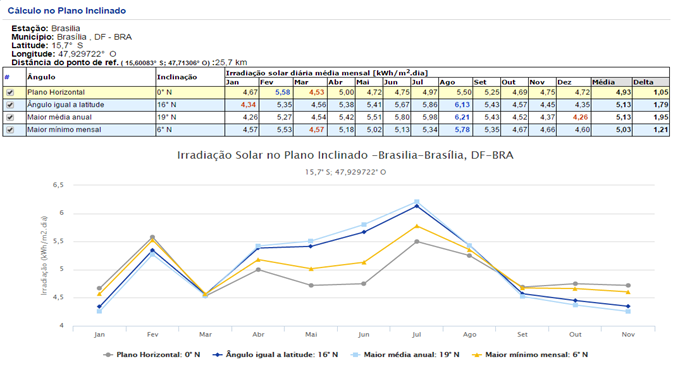
\includegraphics[keepaspectratio=true,scale=0.7]{planejamento/CalculoPlanoInclinado.png}
	\caption{Dados Solarim\'etricos de Bras\'ilia}
	\small{Fonte:  \cite{CRESESBIMAGEM} }
\end{figure}

Utilizando ent\~ao placas de 15\% de efici\^encia em um local que o \'indice solarim\'etrico \'e de 4,57 kWh/m$^{2}$.dia temos que a energia el\'etrica gerada por metro quadrado de placa fotovoltaica em um dia \'e de 685,5 Wh Ent\~ao, em uma \'area de 306,01m$^{2}$ e no per\'iodo de 30 dias seria gerado 6293,1 kWh. Como \'e improv\'avel que 100\% da \'area seja aproveitada, ser\'a descontado 20\% para melhorar a estimativa, que fica 5034,5 kWh. Como a ilumina\c{c}\~ao do parque envolve postes que geram sua pr\'opria energia, tamb\'em com placas solares, essa energia seria utilizada para alimentar a ilumina\c{c}\~ao interna, e pequenos eletrodom\'esticos, e caso haja excedente, redistribu\'ida na rede el\'etrica para a comunidade.

Com isso conclui-se que sem impactos ambientais, e sem a necessidade de construir outras estruturas, a quantidade de energia gerada por pain\'eis fotovoltaicos instalados apenas sobre as edifica\c{c}\^oes m\'inimas do edital de licita\c{c}\~ao, \'e suficiente para abastecer at\'e 30 resid\^encias, admitindo o valor m\'edio de 167 kWh por resid\^encia (Relat\'orio da EPE - Empresa de Pesquisa Energ\'etica). Com isso \'e aceit\'avel dizer que \'e suficiente para abastecer o parque.

\subsection{Coleta Seletiva}

Reduzir, reutilizar e reciclar. \'E com base nesses tr\^es princ\'ipios que percebeu-se a import\^ancia e a viabilidade de se implantar o Programa de Gerenciamento de Res\'iduos S\'olidos (PGRS) no parque urbano da cidade do Gama-DF. Tendo como base a sua implanta\c{c}\~ao no parque tem\'atico \textit{Beto Carrero World} em Santa Catarina no primeiro semestre de 2013. Essa iniciativa faz com que o cuidado com o meio ambiente seja feito por meio do reaproveitamento de materiais atrav\'es da reciclagem.

	O programa prev\^e que \'e responsabilidade todos, separar os res\'iduos, desde o funcion\'ario at\'e o visitante. O programa funciona de forma que torna-se comum o visitante do parque se deparar com duas lixeiras, uma laranja, para res\'iduo recicl\'avel e outra cinza, destinada ao res\'iduo n\~ao recicl\'avel, como por exemplo, os org\^anicos. Al\'em das cores das lixeiras, tamb\'em s\~ao utilizados cores diferentes de sacos de lixo. Desta forma quando os res\'iduos chegam aos bastidores, j\'a se sabe o tipo de res\'iduos e a forma/local de armazenamento.


\subsection{Solu\c{c}\~ao de servi\c{c}os}

Espa\c{c}o lazer multim\'idia, que traga alguma forma de moderniza\c{c}\~ao tecnol\'ogica que torne interessante a realiza\c{c}\~ao de eventos no Parque do Gama.

\subsection{Esportes}

Uma op\c{c}\~ao vi\'avel seria a bicicleta ergom\'etrica que armazene energia para iluminar uma quadra. Entretanto a quest\~ao da viabilidade econ\^omica e de gera\c{c}\~ao de energia foi questionada pelo grupo e nesse sentido pensou-se em uma alternativa de bicicleta (m\'ovel) que tenha uma tecnologia embarcada que mostre em tempo real, dados espec\'ificos do rendimento metab\'olico daquela atividade, podendo ser transmitido para um aplicativo para smartphone/tablet.

\subsubsection{Estudo da viabilidade}

\textit{Wi-Fi} Comunit\'ario: Esse projeto, demanda um custo alto de acordo com a quantidade de \textit{totens} a serem instalados no parque. Estimando um valor pr\'oximo ao valor que a Prefeitura de S\~ao Paulo paga por seus pontos de acesso \textit{Wi-Fi} em pra\c{c}as, ficaria em torno de R\$ 6500,00 por m\^es por \'areas com ponto de acesso, mais os custos iniciais com a instala\c{c}\~ao, considerando que o Parque do Gama tenha \'area correspondente \`a 10 pra\c{c}as da cidade S\~ao Paulo, o custo seria aproximadamente R\$ 65000,00 por m\^es, logo etorno de R\$ 780000,00 ao ano. Um custo vi\'avel, caso o projeto consiga o apoio do Governo do Distrito Federal e/ou empresas patrocinadoras.

	O uso de bicicletas ergom\'etricas sustent\'aveis \'e uma forma de produzir energia el\'etrica limpa. Ela pode ser estacionada ou m\'ovel. Seria uma maneira atrativa, para incentivar os frequentadores do parque a praticarem exerc\'icios com ajuda na concientiza\c{c}\~ao ambiental. Essas bicicletas usadas em grande escala, podem gerar a energia necess\'aria para a ilumina\c{c}\~ao das quadras poli-esportivas por exemplo. Quando m\'ovel, poderia existir um aplicativo de celular para saber quantas calorias, est\~ao sendo perdidas. Essas bicicletas estacionadas j\'a est\'a sendo de grande uso em academias e grandes hot\'eis, pois produz energia el\'etrica de forma limpa.

\subsection{Infraestrutura}

Rede \textit{Wi-Fi} comunit\'aria (o sinal de \textit{Wi-Fi} ser\'a gratuito e de livre acesso, sem necessidade de cadastro, tendo como exemplo o projeto Pra\c{c}as \textit{Wi-Fi} Livre SP, projeto que j\'a est\'a em funcionamento na cidade de S\~ao Paulo, onde a prefeitura instalou pontos de transmiss\~ao \textit{Wi-Fi} gratuitos, com velocidade e 512kbit/s , em v\'arias pra\c{c}as, a adapta\c{c}\~ao que pode ser feita no Parque do Gama, \'e que esses pontos de acesso sejam em \textit{totens}, com tomadas e cabos para carregar os celulares, \textit{tablets} e \textit{notebooks}, como os j\'a utilizados em v\'arios \textit{shoppings}, e velocidade da internet seja de ao menos 1 mega. E esses \textit{totens} seriam localizados em \'areas de maior movimenta\c{c}\~ao do parque). 